\documentclass{beamer}

\mode<presentation>
{
  \usetheme{Singapore}
  \usecolortheme{rose}
  \setbeamercovered{transparent}
}

\usepackage[english]{babel}
\usepackage[latin1]{inputenc}
\usepackage{times}
\usepackage{listings}
\usepackage[T1]{fontenc} 

% Or whatever. Note that the encoding and the font should match. If T1
% does not look nice, try deleting the line with the fontenc.
\usepackage{amsmath}
\newcommand{\linespace}{\vskip 0.25cm}

\definecolor{MyForestGreen}{rgb}{0,0.7,0} 
\newcommand{\tableemph}[1]{{#1}}
\newcommand{\tablewin}[1]{\tableemph{#1}}
\newcommand{\tablemid}[1]{\tableemph{#1}}
\newcommand{\tablelose}[1]{\tableemph{#1}}

\definecolor{MyLightGray}{rgb}{0.6,0.6,0.6}
\newcommand{\tabletie}[1]{\color{MyLightGray} {#1}}

\addtobeamertemplate{navigation symbols}{}{%
    \usebeamerfont{footline}%
    \usebeamercolor[fg]{footline}%
    \hspace{1em}%
    \insertframenumber/\inserttotalframenumber
}

\lstset{language=Java, frame=single, showspaces=false, }

\title[Developmental plasticity in N-gram GP]{Thread Scheduler Efficiency Improvements \\ for Multicore Systems}

% Sub-titles are optional - uncomment and edit the next line if you want one.
% \subtitle{Why does sub-tree crossover work?} 

% The text in square brackets is the short version of your name(s) and will be used in the
% header/footer depending on your theme.
\author[DFrz]{Daniel Collin Frazier}

% The text in square brackets is the short version of your institution and will be used in the
% header/footer depending on your theme.
\institute[U of Minn, Morris]
{
  Division of Science and Mathematics \\
  University of Minnesota, Morris \\
  Morris, Minnesota, USA
}

% The text in square brackets is the short version of the date if you need that.
\date[November '17, UMM, Minnesota] % (optional)
{18 November 2017 \\ UMM, Minnesota}

% Delete this, if you do not want the table of contents to pop up at
% the beginning of each subsection:
\AtBeginSection[]
{
	\begin{frame}<beamer>
		\frametitle{Outline}
		\tableofcontents[currentsection, hideothersubsections]
	\end{frame}
}

\begin{document}

\begin{frame}
\titlepage
\end{frame}

% For a 20-25 minute senior seminar talk you probably want something like:
% - Two or three major sections (other than the summary).
% - At *most* three subsections per section.
% - Talk about 30s to 2min per frame. So there should probably be between
%   15 and 30 frames, all told.

\section*{Introduction}

\subsection*{Introduction}

\begin{frame}
  \frametitle{Introduction}
  
\begin{itemize}
	\item \emph{Thread scheduler} is an important system component that manages the processing programs receive in a given time
  	\item Always running, so it must be efficient
  	
	\linespace
	
 	\item Most computers before 2001 were equipped with one processor containing one core
	\item At the end of the single-processor single-core era (early 2000s) thread scheduling was largely considered a solved problem by the Linux community

\end{itemize}

\end{frame}


\begin{frame}

\begin{figure}

\begin{quote}
``...not very many things that have aged as well as the scheduler. Which is just another proof that scheduling is easy.''
\end{quote}
Linus, Torvals, 2001 \cite{Lozi:2016}
\end{figure}
\end{frame}

\begin{frame}
\frametitle{Introduction}

Hardware changed rapidly throughout the 2000s and those developments made thread scheduler implementation much more complex

\linespace

One of these changes was the development of multicore systems

\end{frame}


\begin{frame}
\frametitle{Introduction}


\begin{columns}
	\begin{column}{0.78\textwidth}

		\begin{itemize}
		\item The computer processor is responsible for executing compiled code.

		\item A single-core processor has one \emph{processing unit}, while a multi-core processor has many \emph{processing units}.

		\item A processing unit contains \emph{registers} which can be seen as a snapshot of the current state of a running program on that processing unit

		\item A processor with multiple cores allows it perform tasks concurrently on each core
		\end{itemize}
	\end{column}
	\begin{column}{0.22\textwidth}
		\begin{figure}
		%{a,e}x are the lower halves of their extended registers.
		%But it's not important that the graphic here accurately represent modern registers, because registers aren't the focus of this talk.
		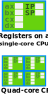
\includegraphics[width=0.95\textwidth]{Illustrations/Registers}
		\label{fig:registers}
		\end{figure}
	\end{column}
\end{columns}
\end{frame}

\subsection*{Outline}

\begin{frame}
  \frametitle{Outline}
  \tableofcontents[hideallsubsections]
\end{frame}

\section[Concepts]{Concepts}

\subsection[Threads]{Threads}

\begin{frame}
\frametitle{Using Threads}

\begin{columns}
	\begin{column}{0.5\textwidth}
		\begin{itemize}
		\item \emph{Threads} allow a program to run multiple independent tasks at the same time
		
		\linespace
		
		\item Useful for programs:
			\begin{itemize}
  			 \item with long, mostly-independent computations
			 \item with a graphical interface
	  		\end{itemize}
		\end{itemize}
	\end{column}
	
	\begin{column}{0.5\textwidth}
		\begin{figure}
		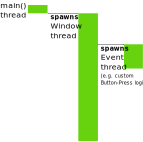
\includegraphics[width=0.95\textwidth]{Illustrations/ThreadExample_GUI}
		\label{fig:domains}
		\caption{Example GUI Program. \textbf{Three} threads are created within \textbf{one} process}
		\end{figure}
	\end{column}
\end{columns}

\end{frame}

\begin{frame}
\frametitle{Using Threads}

	\begin{itemize}
  		\item A \emph{multithreaded} program is a program that employs threads
  		
  		\linespace
  		
  		\item \emph{Concurrent} computing techniques are techniques that allow many tasks to occur at the same time [W]
  		
  		\linespace  		
  		
  		\item \emph{Parallel} computing techniques are techniques that allow many calculations to occur at the same time [W]
  		
  		\linespace  		
  		
  		\item Problems can be solved or improved using neither, either, or both of these techniques at once
	  \end{itemize}

\end{frame}


\begin{frame}
\frametitle{Race Conditions}

One problem multithreaded programs face are called \emph{Race~Conditions}

\linespace

Defined in Saltzer and Kaashoek as ``A timing-dependent error in thread coordination that may result in threads computing incorrect results'' 

\linespace

Let's see an example where two threads increment a shared variable
\end{frame}

\begin{frame}
\frametitle{Race Condition Example}
	\begin{figure}
		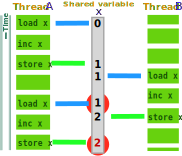
\includegraphics[width=0.8\textwidth]{Illustrations/RaceCondition}
		\label{fig:racecondition}
	\end{figure}

\end{frame}

\subsection[Locks]{Synchronicity and Locks}


\begin{frame}
\frametitle{Synchronicity and Locks}

\begin{itemize}
	\item Race conditions can be fixed by controlling access to shared data.
	\item This control is achieved by employing locks
	
	\linespace
	
	\item \emph{Locks} secure objects or data shared between threads such that only one thread can read and write to it at one time

	\linespace

	\item When a thread \emph{locks} a lock, that thread \textbf{acquires} the lock
	\item When a thread \emph{unlocks} a lock, that thread \textbf{releases} the lock
\end{itemize}

Now, let's fix the race condition in the previous example using locks

\end{frame}

\begin{frame}
\frametitle{Lock Example}
	\begin{figure}
		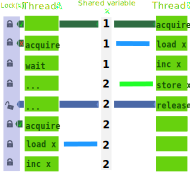
\includegraphics[width=0.7\textwidth]{Illustrations/Lock}
		\label{fig:lock}
	\end{figure}
\end{frame}

\section[Thread Scheduling]{Thread Scheduling on Linux}
\subsection[CFS]{Completely Fair Scheduler}
\begin{frame}
\frametitle{Completely Fair Scheduler (CFS)}

\begin{itemize}
\item Default Linux thread scheduler (there are others)
\item Handles which threads are executed at what times on this core
\item Spend a \emph{fair} amount of runtime on all threads
\end{itemize}

\end{frame}


\begin{frame}
\frametitle{Completely Fair Scheduler (CFS)}

\begin{itemize}
\item Like any program, runs on one core
\item Makes sure all threads run \emph{at least once} within an arbitrary interval of CPU~cycles
\item Distribute \emph{timeslices} (max CPU cycles) among threads
\item Threads with higher priority (weights) get larger timeslices\footnote{Priority (PR) and niceness (NI) values are responsible for determining process priority on Linux. We won't get into that here.}
\item Monitors the number of cycles that the running thread receives and switches it out when it exceeds its timeslice
\end{itemize}

\begin{figure}
		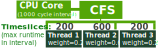
\includegraphics[width=0.8\textwidth]{Illustrations/CFS}
		\label{fig:cfs}
\end{figure}

\linespace

\end{frame}

\begin{frame}
\frametitle{Runqueues}

\begin{itemize}
	\item The data structure within the CFS that contains threads is called a runqueue
	\item A \emph{runqueue} is a priority queue that sorts for threads that have received the least cycles in the current interval
	\item When a thread reaches its maximum time, the first thread in the runqueue is chosen to replace
\end{itemize}

\end{frame}




\begin{frame}
\frametitle{Runqueues on Multiple Cores}
If each core needs work to do, how are threads distributed?

\linespace

Before we can answer this question, we need to know some about switching threads, cache and processor state

\end{frame}



\subsection[Cache]{Thread State and Cache}

\begin{frame}
\frametitle{Context Switching}
\begin{itemize}
\item The scheduler \emph{switches} active threads on cores by saving and restoring thread and processor state information.
\item These switches are called \emph{context switches}
\item Scheduler performance 
\end{itemize}
\end{frame}

\begin{frame}
\frametitle{Process and Thread State}

Process State

\begin{itemize}
	\item[] Consists of resources that each of the processor's threads should have access to
	\item Compiled code, Data
	\item Handles (references) for files and sockets
	\item Process control block (Important logistical information)
\end{itemize}

Thread State

\begin{itemize}
	\item[] Scheduler uses this information to pause and resume a thread's execution
	\item Run-time stack
	\item Copy of core's registers from when the thread was last active
\end{itemize}

\textbf{Important note:} Process state contains much more data

\end{frame}


\begin{frame}
\frametitle{Cache}

\begin{columns}
\begin{column}{0.5\textwidth}
\begin{itemize}
	\item Cache is the fastest form of memory
	\item Memory and cache exists in a hierarchy %POINT ON SLIDE L1, L2, Last-level cache
	\item How cache is arranged depends on the machine:
	\begin{itemize}
		\item A cache can exist \emph{on}, \emph{built-in} to, or \emph{outside} a processor
		\item Cache can be one per \emph{n} processors or one per \emph{n} cores
	
	
	\end{itemize}
\end{itemize}

\end{column}
\begin{column}{0.5\textwidth}
		\begin{figure}
		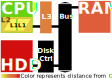
\includegraphics[width=0.95\textwidth]{Illustrations/CacheAbstract}
		\label{fig:domains}
		\caption{Distance of various forms of memory from CPU}
		\end{figure}
	\end{column}
\end{columns}
\end{frame}

\begin{frame}
\frametitle{Cache}

\begin{columns}
\begin{column}{0.5\textwidth}
\begin{itemize}
	\item Cache is the fastest form of memory
	\item \emph{Locality}: Speed of memory read and writes decrease as distance from CPU increases
	
	\linespace
	
	\item \emph{Cache coherence:} Any changes to memory shared by two caches must propogate to the other to maintain correctness
\end{itemize}

\end{column}
\begin{column}{0.5\textwidth}
		\begin{figure}
		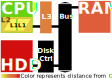
\includegraphics[width=0.95\textwidth]{Illustrations/CacheAbstract}
		\label{fig:domains}
		\caption{Distance of various forms of memory from CPU}
		\end{figure}
	\end{column}
\end{columns}
\end{frame}


\begin{frame}
\frametitle{Runqueues on Multiple Cores (Revisited)}

Since process states are heaver than thread states, context switches between threads of different processes are more expensive

\linespace

\begin{itemize}
	\item If all cores shared one runqueue, access and changes to it would need to be synchronous and cache-coherent
	\item This would slow the system to a crawl
	\item So each core has its own runqueue and threads
\end{itemize}

\linespace

\begin{itemize}
\item In order to best take advantage of available cores, the load on each of the core's runqueues must stay balanced.
\item Most schedulers, including the CFS periodically run a load-balancing algorithm
\item Explaining load-balancing depends on scheduling domains and groups. Don't have time to cover in this talk
\end{itemize}
\end{frame}

\section[Bug Fixes and New Schedulers]{Bug fixes and two new schedulers}
\subsection{CFS Bug Fixes}
\begin{frame}
\frametitle{Bugs everywhere!}

\begin{columns}
\begin{column}{0.72\textwidth}
\begin{itemize}
	\item[] Four bugs from Lozi et al.[W]:
	\item The Overload-on-Wakeup bug
	\item The Missing Scheduling Domains bug
	
	\linespace	
	\noindent\rule{4cm}{0.4pt}
	\linespace	
	
	\item The Scheduling Group Construction bug
	\item The Group Imbalance bug

	\linespace
	
\item[] These two heavily depend on definition of load balancing, scheduling domains, and scheduling groups
	
\end{itemize}
\end{column}
\begin{column}[b]{0.28\textwidth} %Why does to[p] make the figure on the bottom and [b]ottom make the figure on the top.....
\begin{figure}
\centering
\includegraphics[width=0.95\textwidth]{Illustrations/ant_from_pexels.png}
\end{figure}
\end{column}
\end{columns}

\end{frame}


\begin{frame}
\frametitle{The Overload-on Wakeup bug}
\begin{itemize}
\item Optimization in thread wakeup core where threads awakened by other threads are placed on the same core in hope to increase cache locality.

\linespace

\item However, it does this disregarding whether the thread should start on an idle core instead!	
\end{itemize}

\linespace

\begin{itemize}
\item This problem only occurs in environments where threads sleep frequently, such as database systems.
\end{itemize}

\end{frame}


\begin{frame}
\frametitle{The Overload-on Wakeup bug}
The fix for this bug was to modify thread wakeup code:
\linespace

When a thread awakens by another, if the same core isn't busy it will go to that core, otherwise it goes to an idle core

\linespace

Since this bug strongly effected database systems, Lozi et al. ran a database benchmark for a popular proprietary database called TPC-H.

\begin{table}
	\centering
	\begin{tabular}{| c | c | c |}
		\hline			
	  	Bug Fixes & TPC-H request \#18 & Full TPC-H benchmark \\ \hline
		\emph{None} & 55.9s & 542.9s \\ \hline
		\emph{Overload-on-Wakeup} & 43.5s (-22.2\%) & 471.1s (-13.2\%) \\
		\hline
	\end{tabular}
	\caption{"Impact of the bug fixes for Overload-on-Wakeup on a popular commercial database (values averaged after five runs.)"}
\end{table}

\end{frame}

\begin{frame}
\frametitle{The Missing Scheduling Domains bug}

\linespace


\end{frame}


\subsection{Shuffler}
\begin{frame}
\frametitle{Shuffler}

text

\end{frame}

\subsection{FLSched}
\begin{frame}
\frametitle{FLSched}

text

\end{frame}

\section[Conclusions]{Conclusions}

\begin{frame}
\frametitle{Conclusions}

\begin{itemize}
  \item Added developmental plasticity to N-gram GP using Incremental Fitness-based Development (IFD).
\end{itemize}

\begin{itemize}
  \item IFD consistently improved N-gram GP performance on suite of test problems.
  
  \linespace
  
  \item ``Knocking out'' IFD shows it's valuable in all phases, even if it wasn't used earlier in a run.

  \linespace
  
  \item IFD generates more complex, less converged probability tables.
  \item IFD generates more modules/loops \& uses more low-probability paths.
\end{itemize}

\begin{itemize}
  \item Currently exploring applications to dynamic environments.
\end{itemize}

\end{frame}

\begin{frame}
\frametitle{Thanks!}

Thank you for your time and attention!
	
\linespace
\linespace

Contact:  
\begin{itemize}
	\item \texttt{mcphee@morris.umn.edu}
	\item \url{http://www.morris.umn.edu/~mcphee/}
\end{itemize}

\linespace
\linespace

\begin{center}
{\huge Questions?}
\end{center}
\end{frame}

\section*{References}

\begin{frame} 
\frametitle{References} 

\begin{thebibliography}{lskdjf}

%https://www.pexels.com/photo/nature-red-animal-insect-40825/
\bibitem{Jo:2017}
H.~Jo, W.~Kang, C.~Min, and T.~Kim.

\newblock FLsched: A lockless and lightweight approach to OS scheduler for Xeon Phi.

\newblock In G\"unther Raidl, \emph{et al}, editors, {\em GECCO '09}, pages 1019--1026, Montr\'eal, Qu\'ebec, Canada, 2009.

\bibitem{Lozi:2016}
R.~Poli and N.~McPhee.
\newblock A linear estimation-of-distribution {GP} system.
\newblock In M.~O'Neill, \emph{et al}, editors, {\em EuroGP 2008}, volume
  4971 of {\em LNCS}, pages 206--217, Naples,
  26-28 Mar. 2008. Springer.
  
\end{thebibliography}

\linespace
\begin{center}
	See the GECCO '09 paper for additional references.
	\end{center}
\end{frame} 

\end{document}


